\documentclass[border=10pt]{standalone}

\usepackage{tikz}
\usepackage{tikzsymbols}
\usetikzlibrary{calc,patterns,shapes.geometric}

\def\centerarc[#1](#2)(#3:#4:#5){\draw[#1] ($(#2)+({#5*cos(#3)},{#5*sin(#3)})$) arc (#3:#4:#5);}

\begin{document}
	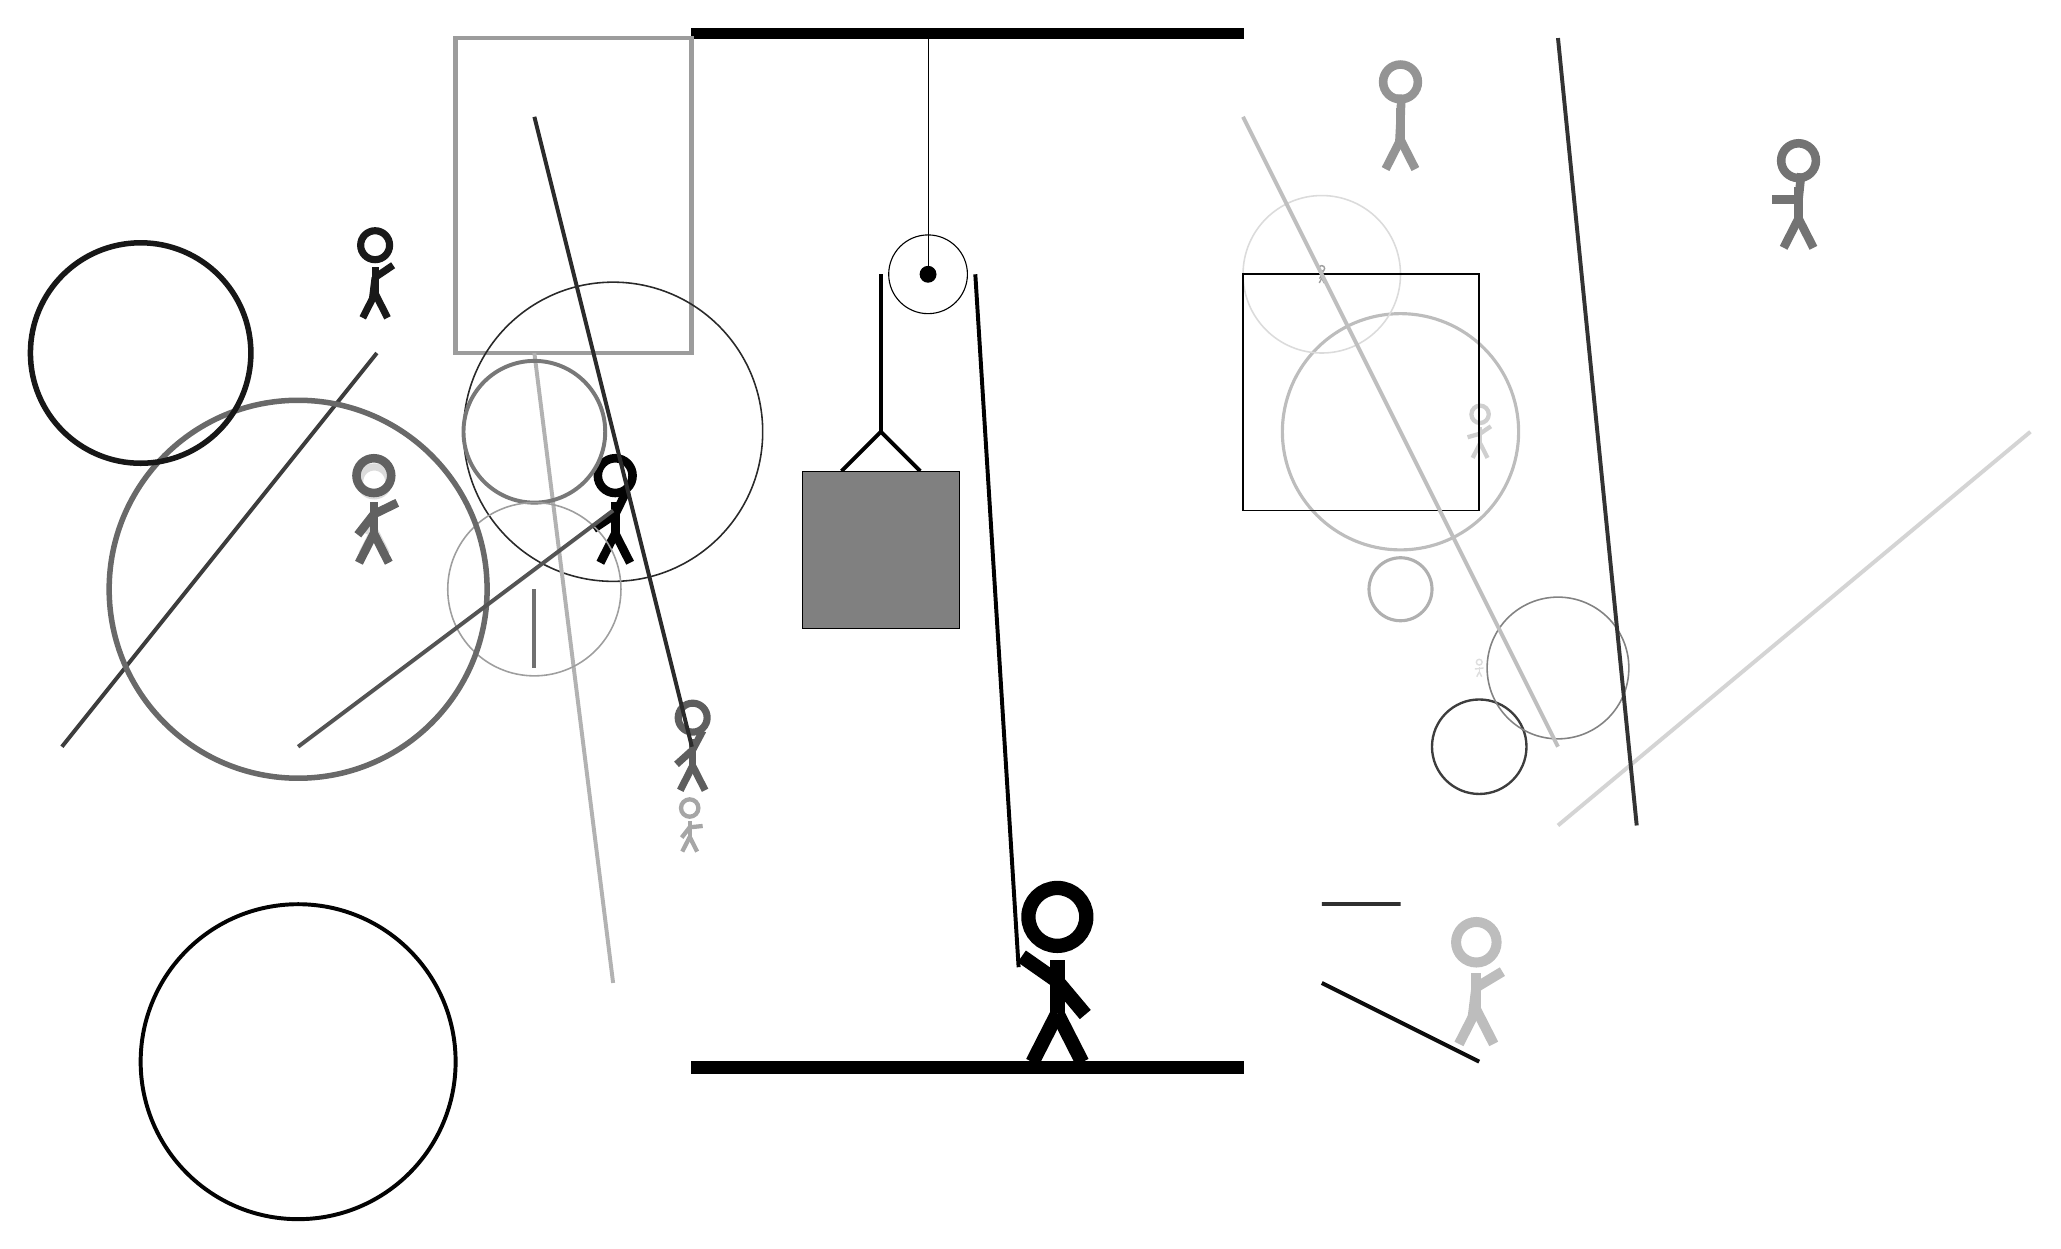
\begin{tikzpicture}
		%%%%% START %%%%%
		
		\draw[fill=black] (-2, 10) rectangle (5, 10.125);
		
		\draw (1, 7) circle (0.5);
		\draw[fill=black] (1, 7) circle (0.1);
		\draw (1, 10) -- (1, 7);
		
		\draw[line width=0.5mm] (-0.1, 4.5) -- (0.4, 5.0) -- (0.9, 4.5);
		\draw[fill=black!50] (-0.6, 4.5) rectangle (1.4, 2.5);
		
		\draw[line width=0.5mm] (0.4, 7) -- (0.4, 5.0);
		\centerarc[line width=0.5mm](1, 7)(0:180:0.6);
		\draw[line width=0.5mm](1.6, 7) -- (2.15, -1.8);
		
		\draw[line width=0.6mm, color=black!39] (-2, 10) rectangle (-5, 6);
		
		\draw [line width=0.2mm, color=black!84](-3, 5) circle (1.9);
		\node[line width=0.2mm, color=black!19] at (8, 5) {\Strichmaxerl[3][16][34]};
		\draw [line width=0.5mm, color=black!99](-7, -3) circle (2.0);
		\node[line width=0.4mm, color=black!26] at (8, -2) {\Strichmaxerl[7][83][31]};
		
		\node[line width=0.3mm, color=black!63] at (-2, 1) {\Strichmaxerl[5][42][62]};
		\node[line width=0.2mm, color=black!38] at (6, 7) {\Strichmaxerl[1][59][70]};
		
		\draw[line width=0.5mm, color=black!81] (7, -1) rectangle (6, -1);
		\node[line width=0.5mm, color=black!99] at (-3, 4) {\Strichmaxerl[6][34][64]};
		\draw[line width=0.5mm, color=black!76](-6, 6) -- (-10, 1);
		\draw [line width=0.4mm, color=black!26](7, 5) circle (1.5);
		\node[line width=0.2mm, color=black!55] at (12, 8) {\Strichmaxerl[6][0][84]};
		\draw[line width=0.5mm, color=black!83](-4, 9) -- (-2, 1);
		
		\draw[line width=0.5mm, color=black!30](-3, -2) -- (-4, 6);
		\draw [line width=0.5mm, color=black!53](-4, 5) circle (0.9);
		\draw[line width=0.5mm, color=black!56](-4, 2) -- (-4, 3);
		
		\draw [line width=0.2mm, color=black!38](-4, 3) circle (1.1);
		
		\draw [line width=0.2mm, color=black!14](6, 7) circle (1.0);
		\draw[line width=0.5mm, color=black!17](9, 0) -- (15, 5);
		\draw [line width=0.3mm, color=black!76](8, 1) circle (0.6);
		\draw [line width=0.2mm, color=black!49](9, 2) circle (0.9);
		
		\node[line width=0.5mm, color=black!14] at (-6, 4) {\Strichmaxerl[5][70][24]};
		\node[line width=0.3mm, color=black!90] at (-6, 7) {\Strichmaxerl[5][83][34]};
		\node[line width=0.2mm, color=black!62] at (-6, 4) {\Strichmaxerl[6][52][26]};
		\draw [line width=0.7mm, color=black!59](-7, 3) circle (2.4);
		
		\node[line width=0.5mm, color=black!42] at (7, 9) {\Strichmaxerl[6][87][88]};
		\draw[line width=0.5mm, color=black!95](8, -3) -- (6, -2);
		\draw [line width=0.7mm, color=black!91](-9, 6) circle (1.4);
		\draw [line width=0.4mm, color=black!31](7, 3) circle (0.4);
		
		\draw[line width=0.5mm, color=black!67](-3, 4) -- (-7, 1);
		\draw[line width=0.2mm, color=black!99] (5, 7) rectangle (8, 4);
		
		\draw[line width=0.5mm, color=black!25](5, 9) -- (9, 1);
		\node[line width=0.7mm, color=black!35] at (-2, 0) {\Strichmaxerl[3][52][6]};
		
		\draw[line width=0.5mm, color=black!80](9, 10) -- (10, 0);
		
		\node[line width=0.2mm, color=black!13] at (8, 2) {\Strichmaxerl[1][4][9]};
		
		\node at (2.6, -1.9) {\Strichmaxerl[10][-35][-50]};
		
		\draw[fill=black] (-2, -3) rectangle (5, -3.15);
		
		%%%%% END %%%%%
	\end{tikzpicture}
\end{document}